\documentclass[12pt,twoside,a4paper]{report}
\usepackage[a4paper,width=150mm,top=25mm,bottom=25mm,bindingoffset=6mm]{geometry}

\usepackage[utf8x]{inputenc}
\usepackage[slovak]{babel}
\usepackage{palatino,verbatim}

% Balicek pre priamu rec - \say
\usepackage{dirtytalk}

% Balicek "alltt" je to iste ako "verbatim" mod, ale navyse podporuje aj formatovacie znacky textu
\usepackage{alltt}

% Obrazky
\usepackage{graphicx}
\graphicspath{ {obr/} }

% Cislovanie obrazkov a tabuliek
\usepackage{chngcntr}
%Cisluj obrazky nezavisle od cisla kapitol/podkapitol
\counterwithout{figure}{subsection}
\counterwithout{table}{subsection}

% Referencovanie kapitol/sekcii/... podľa ich nadpisu
\usepackage{nameref}

% Tabulky s viacriadkovymi bunkami a zlucenymi bunkami
% Tabulky generujem naastrojom "http://www.tablesgenerator.com/"
\usepackage{booktabs}
\usepackage{multirow}
% LaTeX ma problemy s prikazmi cline a cmidrule, ked je babel nastaveny na slovencinu/cestinu, kvoli definicii pomlcky
% NAMIESTO POMLCKY POUZI ZNAK ZNAMIENKA MINUS "−" (plati hlavne v nazvoch nadpisov a labelov)
\usepackage{etoolbox}
\preto\tabular{\shorthandoff{-}}

%Uloz obrazok tam, kde je deklarovany
%\usepackage[subsection]{placeins}

\newcommand\sktxt[1]{\foreignlanguage{slovak}{#1}}

\begin{document}
\pagenumbering{arabic}

\setcounter{chapter}{1}
\chapter*{Internet Peering}
\paragraph{}
Andrej Šišila, Marián Vachalík

\tableofcontents

\newpage
\section{Topológia}
\paragraph{}
Budeme konfigurovať smerovacie protokoly BGP a IS-IS na topológií, ktorá je znázornená na obrázku \ref{fig:bgp_isis_topo}. Vrámci autonómnych systémov sme konfigurovali smerovacie protokoly IS-IS a BGP (iBGP). Medzi autonómnymi systémami sme konfigurovali len BGP (eBGP). IP adresácia je uvedená v tabuľke \ref{tab:ip_adresacia} a dopĺňa grafické znázornenie topológie na obrázku \ref{fig:bgp_isis_topo}. Sieť medzi smerovačmi R1 a R5 nemá mať masku \say{/48} ale \say{/30}.

\begin{figure}[!htbp]
\centering
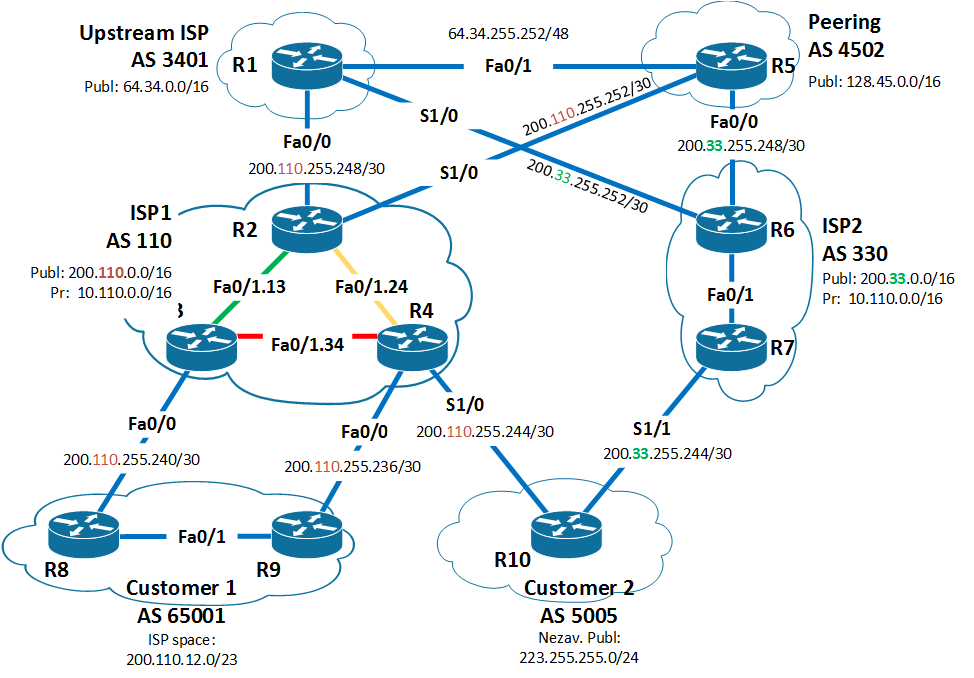
\includegraphics[width=14cm,keepaspectratio]{bgp_isis_topo}
\caption{Topológia BGP}
\label{fig:bgp_isis_topo}
\end{figure}



\begin{table}[!htbp]
\centering
\caption{IP adresácia}
\label{tab:ip_adresacia}
\begin{tabular}{|c|l|l|l|}
\hline
\textbf{Smerovač}    & \multicolumn{1}{c|}{\textbf{Rozhranie}} & \multicolumn{1}{c|}{\textbf{IP adresa}} & \multicolumn{1}{c|}{\textbf{Maska}} \\ \hline
\multirow{5}{*}{R1}  & Fa0/0                                   & 200.110.255.249                         &                                     \\ \cline{2-4} 
                     & Fa0/1                                   & 64.34.255.253                           &                                     \\ \cline{2-4} 
                     & S1/0                                    & 200.33.255.253                          &                                     \\ \cline{2-4} 
                     & Lo0                                     & 10.255.255.1                            & 255.255.255.255                     \\ \cline{2-4} 
                     & Lo1                                     & 64.34.1.1                               &                                     \\ \hline
\multirow{5}{*}{R2}  & Fa0/0                                   & 200.110.255.250                         &                                     \\ \cline{2-4} 
                     & Fa0/1.23                                & 10.110.23.2                             &                                     \\ \cline{2-4} 
                     & Fa0/1.24                                & 10.110.24.2                             &                                     \\ \cline{2-4} 
                     & S1/0                                    & 200.110.255.253                         &                                     \\ \cline{2-4} 
                     & Lo0                                     & 10.255.255.2                            & 255.255.255.255                     \\ \hline
\multirow{4}{*}{R3}  & Fa0/0                                   & 200.110.255.241                         &                                     \\ \cline{2-4} 
                     & Fa0/1.23                                & 10.110.23.3                             &                                     \\ \cline{2-4} 
                     & Fa0/1.34                                & 10.110.34.3                             &                                     \\ \cline{2-4} 
                     & Lo0                                     & 10.255.255.3                            & 255.255.255.255                     \\ \hline
\multirow{5}{*}{R4}  & Fa0/0                                   & 200.110.255.237                         &                                     \\ \cline{2-4} 
                     & Fa0/1.24                                & 10.110.24.4                             &                                     \\ \cline{2-4} 
                     & Fa0/1.34                                & 10.110.34.4                             &                                     \\ \cline{2-4} 
                     & S1/0                                    & 200.110.255.245                         &                                     \\ \cline{2-4} 
                     & Lo0                                     & 10.255.255.4                            & 255.255.255.255                     \\ \hline
\multirow{5}{*}{R5}  & Fa0/0                                   & 200.33.255.249                          &                                     \\ \cline{2-4} 
                     & Fa0/1                                   & 10.100.15.2                             &                                     \\ \cline{2-4} 
                     & S1/0                                    & 200.110.255.254                         &                                     \\ \cline{2-4} 
                     & Lo0                                     & 10.255.255.5                            & 255.255.255.255                     \\ \cline{2-4} 
                     & Lo1                                     & 128.45.5.1                              &                                     \\ \hline
\multirow{5}{*}{R6}  & Fa0/0                                   & 200.33.255.250                          &                                     \\ \cline{2-4} 
                     & Fa0/1                                   & 10.110.67.6                             &                                     \\ \cline{2-4} 
                     & S1/0                                    & 200.33.255.254                          &                                     \\ \cline{2-4} 
                     & Lo0                                     & 10.255.255.6                            & 255.255.255.255                     \\ \cline{2-4} 
                     & Lo1                                     & 200.33.6.1                              &                                     \\ \hline
\multirow{4}{*}{R7}  & Fa0/1                                   & 10.110.67.7                             &                                     \\ \cline{2-4} 
                     & S1/1                                    & 200.33.255.245                          &                                     \\ \cline{2-4} 
                     & Lo0                                     & 10.255.255.7                            & 255.255.255.255                     \\ \cline{2-4} 
                     & Lo1                                     & 200.33.7.1                              &                                     \\ \hline
\multirow{4}{*}{R8}  & Fa0/0                                   & 200.110.255.242                         &                                     \\ \cline{2-4} 
                     & Fa0/1                                   & 10.110.89.8                             &                                     \\ \cline{2-4} 
                     & Lo0                                     & 10.255.255.8                            & 255.255.255.255                     \\ \cline{2-4} 
                     & Lo1                                     & 200.110.12.1                            &                                     \\ \hline
\multirow{4}{*}{R9}  & Fa0/0                                   & 200.110.255.238                         &                                     \\ \cline{2-4} 
                     & Fa0/1                                   & 10.110.89.9                             &                                     \\ \cline{2-4} 
                     & Lo0                                     & 10.255.255.9                            & 255.255.255.255                     \\ \cline{2-4} 
                     & Lo1                                     & 200.110.13.1                            &                                     \\ \hline
\multirow{4}{*}{R10} & S1/0                                    & 200.110.255.246                         &                                     \\ \cline{2-4} 
                     & S1/1                                    & 200.33.255.246                          &                                     \\ \cline{2-4} 
                     & Lo0                                     & 10.255.255.10                           & 255.255.255.255                     \\ \cline{2-4} 
                     & Lo1                                     & 223.255.255.1                           &                                     \\ \hline
\end{tabular}
\end{table}


% Novu kapitolu davam na novu stranu, lebo bez toho mi zobrazuje tabulku v dalsej kapitole, kde ale tabulka nepatri.
\newpage

\section{Úlohy}
\subsection{Použiť IGP IS−IS (L2 only) single area dizajn, priame p2p prepojenia}


\subsubsection{Popis}
Dohodli sme sa, že vnútri autonómneho systému budeme používať iba smerovací protokol IS-IS. Medzi autonómnymi systémami používame smerovací protokol BGP. Subrozhranie “.13” a VLAN 13 sme premenovali na “.23” a VLAN 23, lebo sieť je medzi smerovačmi R2 a R3 (23), a nie medzi R1 a R3 (13).


\subsubsection{Konfigurácia}

\noindent
{\fontfamily{qcr}\selectfont
\begin{small}
\begin{alltt}
R1
ena
conf t
hostname R1
no ip domain-lookup
username admin privil 15 secret admin
line con 0
  login local
  logging syn
  exec-time 120
line vty 0 15
  privilege level 15
  no login
int f0/0
  ip addr 200.110.255.249 255.255.255.252
  no shut
int f0/1
  ip addr 64.34.255.253 255.255.255.252
  no shut
int s1/0
  ip addr 200.33.255.253 255.255.255.252
  no shut
int lo0
  ip addr 10.255.255.1 255.255.255.255
  no shut
int lo1
  ip addr 64.34.1.1 255.255.255.0
  no shut
router bgp 3401
  neighbor 64.34.255.254 remote-as 4502
  neighbor 200.33.255.254 remote-as 330
  neighbor 200.110.255.250 remote-as 110
  network 10.255.255.1 mask 255.255.255.255
  no auto-summary
  no sync
  bgp log-neighbor-changes



R2
ena
conf t
hostname R2
no ip domain-lookup
username admin privil 15 secret admin
line con 0
  login local
  logging syn
  exec-time 120
line vty 0 15
  privilege level 15
  no login
int f0/0
  ip addr 200.110.255.250 255.255.255.252
  no shut
int f0/1
  no ip add
  isis network point-to-point
  no sh
int f0/1.23
  encap dot1q 23
  ip addr 10.110.23.2 255.255.255.0
  ip router isis
int f0/1.24
  encap dot1q 24
  ip addr 10.110.24.2 255.255.255.0
  ip router isis
int s1/0
  ip addr 200.110.255.253 255.255.255.252
  no shut
int lo0
  ip addr 10.255.255.2 255.255.255.255
  ip router isis
  no shut
router isis
  net 49.0001.0102.5525.5002.00
  passive-interface lo0
  passive-interface f0/0
  redistribute static
  redistribute connected
  is-type level-2
  metric-style wide
  exit
router bgp 110
  neighbor 10.255.255.3 remote-as 110
  neighbor 10.255.255.3 update-source lo0
  neighbor 10.255.255.4 remote-as 110
  neighbor 10.255.255.4 update-source lo0
  neighbor 200.110.255.249 remote-as 3401
  neighbor 200.110.255.254 remote-as 4502
  network 10.255.255.2 mask 255.255.255.255
  no auto-summary
  no sync
  bgp log-neighbor-changes



R3
ena
conf t
hostname R3
no ip domain-lookup
username admin privil 15 secret admin
line con 0
  login local
  logging syn
  exec-time 120
line vty 0 15
  privilege level 15
  no login
int f0/0
  ip addr 200.110.255.241 255.255.255.252
  no shut
int f0/1
  no ip addr
  isis network point-to-point
  no shut
int f0/1.23
  encap dot1q 23
  ip addr 10.110.23.3 255.255.255.0
  ip router isis
int f0/1.34
  encap dot1q 34
  ip addr 10.110.34.3 255.255.255.0
  ip router isis
int lo0
  ip addr 10.255.255.3 255.255.255.255
  ip router isis
  no shut
router isis
  net 49.0001.0102.5525.5003.00
  passive-interface lo0
  passive-interface f0/0
  redistribute static
  redistribute connected
  is-type level-2
  metric-style wide
  exit
router bgp 110
  neighbor 10.255.255.2 remote-as 110
  neighbor 10.255.255.2 update-source lo0
  neighbor 10.255.255.4 remote-as 110
  neighbor 10.255.255.4 update-source lo0
  neighbor 200.110.255.242 remote-as 65001
  network 10.255.255.3 mask 255.255.255.255
  no auto-summary
  no sync
  bgp log-neighbor-changes




R4
ena
conf t
hostname R4
no ip domain-lookup
username admin privil 15 secret admin
line con 0
  login local
  logging syn
  exec-time 120
line vty 0 15
  privilege level 15
  no login
int f0/0
  ip addr 200.110.255.237 255.255.255.252
  no shut
int f0/1
  no ip addr
  isis network point-to-point
  no sh
int f0/1.24
  encap dot1q 24
  ip addr 10.110.24.4 255.255.255.0
  ip router isis
int f0/1.34
  encap dot1q 34
  ip addr 10.110.34.4 255.255.255.0
  ip router isis
int s1/0
  ip addr 200.110.255.245 255.255.255.252
  no shut
int lo0
  ip addr 10.255.255.4 255.255.255.255
  ip router isis
  no shut
router isis
  net 49.0001.0102.5525.5004.00
  passive-interface lo0
  passive-interface f0/0
  passive-interface s1/0
  redistribute static
  redistribute connected
  is-type level-2
  metric-style wide
  exit
router bgp 110
  neighbor 10.255.255.2 remote-as 110
  neighbor 10.255.255.2 update-source lo0
  neighbor 10.255.255.3 remote-as 110
  neighbor 10.255.255.3 update-source lo0
  neighbor 200.110.255.238 remote-as 65001
  neighbor 200.110.255.246 remote-as 5005
  network 10.255.255.4 mask 255.255.255.255
  no auto-summary
  no sync
  bgp log-neighbor-changes


R5
ena
conf t
hostname R5
no ip domain-lookup
username admin privil 15 secret admin
line con 0
  login local
  logging syn
  exec-time 120
line vty 0 15
  privilege level 15
  no login
int f0/0
  ip addr 200.33.255.249 255.255.255.252
  no shut
int f0/1
  ip addr 64.34.255.254 255.255.255.252
  no shut
int s1/0
  ip addr 200.110.255.254 255.255.255.252
  no shut
int lo0
  ip addr 10.255.255.5 255.255.255.255
  no shut
int lo1
  ip addr 128.45.5.1 255.255.255.0
  no shut
router bgp 4502
  neighbor 200.33.255.250 remote-as 330
  neighbor 200.110.255.253 remote-as 110
  neighbor 64.34.255.253 remote-as 3401
  network 10.255.255.5 mask 255.255.255.255
  no auto-summary
  no sync
  bgp log-neighbor-changes




R6
ena
conf t
hostname R6
no ip domain-lookup
username admin privil 15 secret admin
line con 0
  login local
  logging syn
  exec-time 120
line vty 0 15
  privilege level 15
  no login
int f0/0
  ip addr 200.33.255.250 255.255.255.252
  no shut
int f0/1
  ip addr 10.110.67.6 255.255.255.0
  ip router isis
  isis network point-to-point
  no shut
int s1/0
  ip addr 200.33.255.254 255.255.255.252
  no shut
int lo0
  ip addr 10.255.255.6 255.255.255.255
  ip router isis
  no shut
int lo1
  ip add 200.33.6.1 255.255.255.0
  ip router isis
router isis
  net 49.0001.0102.5525.5006.00
  passive-interface lo0
  passive-interface lo1
  passive-interface f0/0
  passive-interface s1/0
  redistribute static
  redistribute connected
  is-type level-2
  metric-style wide
  exit
router bgp 330
  neighbor 10.255.255.7 remote-as 330
  neighbor 10.255.255.7 update-source lo0
  neighbor 200.33.255.253 remote-as 3401
  neighbor 200.33.255.249 remote-as 4502
  network 10.255.255.6 mask 255.255.255.255
  no auto-summary
  no sync
  bgp log-neighbor-changes



R7
ena
conf t
hostname R7
no ip domain-lookup
username admin privil 15 secret admin
line con 0
  login local
  logging syn
  exec-time 120
line vty 0 15
  privilege level 15
  no login
int f0/1
  ip addr 10.110.67.7 255.255.255.0
  ip router isis
  isis network point-to-point
  no shut
int s1/1
  ip addr 200.33.255.245 255.255.255.252
  no shut
int lo0
  ip addr 10.255.255.7 255.255.255.255
  ip router isis
  no shut
int lo1
  ip addr 200.33.7.1 255.255.255.0
  ip router isis
  no shut
router isis
  net 49.0001.0102.5525.5007.00
  passive-interface lo0
  passive-interface lo1
  passive-interface s1/1
  redistribute static
  redistribute connected
  is-type level-2
  metric-style wide
  exit
router bgp 330
  neighbor 10.255.255.6 remote-as 330
  neighbor 10.255.255.6 update-source lo0
  neighbor 200.33.255.246 remote-as 5005
  network 10.255.255.7 mask 255.255.255.255
  no auto-summary
  no sync
  bgp log-neighbor-changes




R8
ena
conf t
hostname R8
no ip domain-lookup
username admin privil 15 secret admin
line con 0
  login local
  logging syn
  exec-time 120
line vty 0 15
  privilege level 15
  no login
int f0/0
  ip addr 200.110.255.242 255.255.255.252
  no shut
int f0/1
  ip addr 10.110.89.8 255.255.255.0
  Ip router isis
  isis network point-to-point
  no shut
int lo0
  ip addr 10.255.255.8 255.255.255.255
  ip router isis
  no shut
int lo1
  ip add 200.110.12.1 255.255.255.0
  ip router isis
router isis
  net 49.0001.0102.5525.5008.00
  passive-interface lo0
  passive-interface lo1
  passive-interface f0/0
  redistribute static
  redistribute connected
  is-type level-2
  metric-style wide
  exit
router bgp 65001
  neighbor 10.255.255.9 remote-as 65001
  neighbor 10.255.255.9 update-source lo0
  neighbor 200.110.255.241 remote-as 110
  network 10.255.255.8 mask 255.255.255.255
  network 200.110.12.0 mask 255.255.255.0
  no auto-summary
  no sync
  bgp log-neighbor-changes





R9
ena
conf t
hostname R9
no ip domain-lookup
username admin privil 15 secret admin
line con 0
  login local
  logging syn
  exec-time 120
line vty 0 15
  privilege level 15
  no login
int f0/0
  ip addr 200.110.255.238 255.255.255.252
  no sh
int f0/1
  ip addr 10.110.89.9 255.255.255.0
  ip router isis
  isis network point-to-point
  no shut
int lo0
  ip addr 10.255.255.9 255.255.255.255
  ip router isis
  no shut
int lo1
  ip addr 200.110.13.1 255.255.255.0
  ip router isis
  no shut
router isis
  net 49.0001.0102.5525.5009.00
  passive-interface lo0
  passive-interface lo1
  passive-interface f0/0
  redistribute static
  redistribute connected
  is-type level-2
  metric-style wide
  exit
router bgp 65001
  neighbor 10.255.255.8 remote-as 65001
  neighbor 10.255.255.8 update-source lo0
  neighbor 200.110.255.237 remote-as 110
  network 10.255.255.9 mask 255.255.255.255
  network 200.110.13.0 mask 255.255.255.0
  no auto-summary
  no sync
  bgp log-neighbor-changes




R10
ena
conf t
hostname R10
no ip domain-lookup
username admin privil 15 secret admin
line con 0
  login local
  logging syn
  exec-time 120
line vty 0 15
  privilege level 15
  no login
int s1/0
  ip addr 200.110.255.246 255.255.255.252
  no shut
int s1/1
  ip addr 200.33.255.246 255.255.255.252
  ip router isis
  no shut
int lo0
  ip addr 10.255.255.10 255.255.255.255
  no shut
int lo1
  ip addr 223.255.255.1 255.255.255.0
  no shut
router bgp 5005
  neighbor 200.110.255.245 remote-as 110
  neighbor 200.33.255.245 remote-as 330
  network 10.255.255.10 mask 255.255.255.255
  network 223.255.255.0 mask 255.255.255.0
  no auto-summary
  no sync
  bgp log-neighbor-changes

\end{alltt}
\end{small}
}

\subsubsection{Overenie}



\subsection{Zabezpečiť plnú konektivitu prostredníctvom iBGP alebo eBGP protokolov pre zákaznícké a internetové smerovacie záznamy}
\subsection{Distribúcia internetových statických smerovacích záznamov z AS3401, AS4502 a zákaznických smerovacích záznamov z AS65001, AS5005, AS330}
\subsection{Prepísať privátne AS65001}
\subsection{Sumarizácia}
\subsection{Kontrola, či interné ISP adresy nie sú propagované}
\subsection{Kontrola konektivity medzi zákazníckymi a internetovými smerovacími záznamami}

\subsection{ISP politika}
\subsection{Definovať vlastnú politiku − použiť community, community alter LP, AS−PATH filtering, prepending, atď}
\subsection{Primárne linky R3−R8, R4−R10}
\subsection{Distribuovať iba default, AS5005 a peering prefixy do AS65001}
\subsection{AS5005 nesme byť nikdy transit}
\subsection{Peering iba pre ISP1 a ISP2, nie pre prefixy naučené z Upstream ISP}
\subsection{Overiť funkčnosť nastavenia politiky vhodnými výpadkami liniek a smerovačov}
\subsection{Overiť, či je možné odkloniť celú prevádzku (upstream, downstream) na linke R4−R10 v prípade plánovanej údržby (linka musí byť plne funkčna a BGP spojenie propaguje všetky prefixy)}


\end{document}